\documentclass{article}
\usepackage[utf8]{inputenc}
\usepackage{amsmath}
\usepackage{amssymb}
\usepackage{indentfirst}
\usepackage{color}
\usepackage{forest}
\usepackage{fancyhdr}
\usepackage{algorithm}
\usepackage{bm}
\usepackage[noend]{algpseudocode}
\usepackage{geometry}
\usepackage[T1]{fontenc}
\geometry{left=2.5cm,right=2.5cm,top=2.5cm,bottom=2.5cm}

\title{6.046/18.410 Problem Set 8}
\author{Yijun Jiang\vspace{3pt}\\Collaborator: Hengyun Zhou, Eric Lau}
%\email{yjjiang@mit.edu}
\date{\today}

\pagestyle{fancy}
\lhead{Yijun Jiang}
\rhead{6.046/18.410 Problem Set 8}

\begin{document}
\maketitle

\section{More Fun with Clam Calamity}
\subsection{Part (a)}
\noindent\textbf{Proof}: Let the $j$-th clam (denoted by $C_j$) has wealth $w_j$, where $j=1,2,\cdots,m$. Since OPT is the wealth of the richest clam, $w_j\leqslant\textup{OPT}$ for all $j$. Therefore, if
\begin{equation*}
\textup{OPT}<\frac{1}{m}\sum_{i=1}^np_i
\end{equation*}
it follows that
\begin{equation*}
\sum_{j=1}^mw_j\leqslant m\textup{OPT}<\sum_{i=1}^np_i
\end{equation*}
which is impossible since the total wealth of clams should equal the total value of pearls. Therefore, it must be that
\begin{equation*}
\textup{OPT}\geqslant\frac{1}{m}\sum_{i=1}^np_i
\end{equation*}

\subsection{Part (b)}
\noindent\textbf{Description}: Take the list of pearls in arbitrary order. For each pearl in this list, give it to the currently poorest clam (break ties arbitrarily). Do this until all the pearls are distributed to the clams.

~

\noindent\textbf{Runtime}: There are $n$ pearls, which correspond to $n$ iterations. In each iteration, naively choosing the poorest clam costs $O(m)$ time. Therefore, the overall runtime is $T=O(mn)$, which is a polynomial of input size.

~

\noindent\textbf{Proof of being 2-approximation}: We first prove by contradiction that the poorest clam has wealth at most $(\sum_{i=1}^np_i)/m$. Suppose this does not hold. Let the poorest clam has wealth $w_{\min}$, then
\begin{equation*}
\sum_{j=1}^mw_j\geqslant mw_{\min}>\sum_{i=1}^np_i
\end{equation*}
which is impossible since the total wealth of clams should equal the total value of pearls.

We also show that OPT is no less than any pearl's value. This is simply because, for any given pearl, whichever clam taking it has wealth at least equal to its value. And this clam's wealth cannot exceed OPT.

Now consider the richest clam after this approximation algorithm. WLOG, let it be $C_1$. It must have at least one pearl. Consider the last pearl that it obtains. Let it be the $r$-th pearl in the list. By the algorithm, just before $C_1$ got this pearl, it was the poorest clam with wealth denoted by $w_{\textup{pre}}$. By the discussion above,
\begin{equation*}
w_{\textup{pre}}\leqslant\frac{1}{m}\sum_{i=1}^{r-1}p_i\leqslant\frac{1}{m}\sum_{i=1}^np_i\leqslant\textup{OPT}
\end{equation*}

Therefore, the richest clam's wealth, denote by $w_{\max}$, is
\begin{equation*}
w_{\max}=w_{\textup{pre}}+p_r\leqslant\textup{OPT}+\textup{OPT}=2\textup{OPT}
\end{equation*}

This shows that the algorithm is a 2-approximation.

\subsection{Part (c)}
\noindent\textbf{Description}: Take the list of pearls and sort it in decreasing order. For each pearl in this list, give it to the currently poorest clam (break ties arbitrarily). Do this until all the pearls are distributed to the clams.

~

\noindent\textbf{Runtime}: Sorting the pearls takes $O(n\log n)$ time. Once the pearls are sorted, $n$ iterations are performed. In each iteration, naively choosing the poorest clam costs $O(m)$ time. Therefore, the overall runtime is $T=O(n\log n+mn)$, which is a polynomial of input size.

~

\noindent\textbf{Proof of being 4/3-approximation}: Still consider the richest clam after this approximation algorithm. WLOG, let it be $C_1$. It must have at least one pearl. Consider the last pearl that it obtains. \textbf{We claim that it suffices to consider the case where this pearl is the last one (the $\bm{n}$-th) in the list.} This is because, if this pearl is actually the $r$-th one, the algorithm distributes the $(r+1)$-th to the $n$-th pearl to clams other than $C_1$, but none of their wealths can exceed the wealth of $C_1$. Think of a new list of pearls $P'$ containing only the first $r$ pearls in the original list $P$. The algorithm will return the same maximum wealth given $P'$ as given $P$. Let the optimal maximum wealth given $P'$ be $\textup{OPT}'$. Since $P'\subset P$, $\textup{OPT}'\leqslant\textup{OPT}$. Therefore, if we can show that the maximum wealth is bounded by $4\textup{OPT}'/3$, it must also be bounded by $4\textup{OPT}/3$. As a result, the subsequent proof focuses on the case where the last pearl in the list is given to the clam that eventually becomes the richest. WLOG, let it be $C_1$.

By the algorithm, just before $C_1$ got the last pearl, it was the poorest clam with wealth denoted by $w_{\textup{pre}}$. By the discussion above,
\begin{equation*}
w_{\textup{pre}}\leqslant\frac{1}{m}\sum_{i=1}^{n-1}p_i\leqslant\frac{1}{m}\sum_{i=1}^np_i\leqslant\textup{OPT}
\end{equation*}

Now consider two cases for the last pearl: (1) $p_n\leqslant\textup{OPT}/3$ and (2) $p_n>\textup{OPT}/3$. In the first case, the wealth of the richest clam is
\begin{equation*}
w_{\max}=w_{\textup{pre}}+p_n\leqslant\textup{OPT}+\frac{1}{3}\textup{OPT}=\frac{4}{3}\textup{OPT}
\end{equation*}
And in the second case, we prove below that the approximation algorithm actually gives the optimal distribution.

~

\noindent\underline{Proof}:
If $n\leqslant m$, in the approximation algorithm, a clam gets either one or no pearl. $w_{\max}$ is thus the most expensive pearl $p_1$. Since from the discussion above, $p_1\leqslant\textup{OPT}$, it must be that $w_{\max}=p_1=\textup{OPT}$.

If $n>m$, we prove optimality by contradiction. Suppose the approximation algorithm gives a $w_{\max}$ strictly larger than OPT. Then there must be a clam whose possession of a certain pearl increases the maximum wealth from no more than OPT to exceeding OPT. Let this pearl be the $r$-th one in the list.

Since the list is sorted in reverse order, $p_r\geqslant p_n>\textup{OPT}/3$. Moreover, all the pearls distributed prior to the $r$-th are no cheaper than $\textup{OPT}/3$. Since before distributing the $r$-th pearl, the maximum wealth did not exceed OPT, at that time a clam could not have more than 2 pearls, otherwise its wealth would exceed OPT. Moreover, before distributing the $r$-th pearl, every clam must have at least one pearl, otherwise the $r$-th pearl would be given to a clam with no pearls, which would not drive the maximum wealth above OPT.

Therefore, prior to the $r$-th pearl, each clam has either one or two pearls. WLOG, let $C_1,C_2,\cdots,C_s$ have one pearl and $C_{s+1},C_{s+2},\cdots,C_m$ have two pearls. Call the pearls owned by $C_1,C_2,\cdots,C_s$ ``Expensive Pearls'' and the pearls owned by $C_{s+1},C_{s+2},\cdots,C_m$, as well as the $r$-th pearl, ``Cheap Pearls''. There are $s$ Expensive Pearls and $2(m-s)+1$ Cheap Pearls. Since the poorest clam's wealth exceeds OPT after obtaining the $r$-th pearl, the wealth of any clam with an Expensive Pearl would also exceed OPT if they had the $r$-th pearl. Moreover, since all pearls prior to the $r$-th are no cheaper, we conclude that in the optimal distribution, a clam that has an Expensive Pearl cannot own any other pearl among the first $r$ of the list.

Therefore, the optimal distribution must select $s$ clams and give each of them an Expensive Pearl. And the $2(m-s)+1$ Cheap Pearls belong to the rest $m-s$ clams. Therefore, at least one clam gets more than than two Cheap Pearls. Since each Cheap Pearl has value greater than $\textup{OPT}/3$, this clam's wealth exceeds OPT. This contradicts to the optimality of the distribution.

As a result, the approximation algorithm cannot give a $w_{\max}$ strictly larger than OPT. Therefore, the approximation algorithm must give the optimal distribution.

\rightline{\underline{QED}}

In conclusion,
\begin{enumerate}
\item{If $p_n\leqslant\textup{OPT}/3$, then $w_{\max}\leqslant4\textup{OPT}/3$.}
\item{If $p_n>\textup{OPT}/3$, then $w_{\max}=\textup{OPT}$.}
\end{enumerate}

This shows that the algorithm is a 4/3-approximation.

\section{Sandwich Shop}
\subsection{Part (a)}
Suppose $x$ units of Monte Cristo sauce and $y$ units of Barbeque sauce are used. Then
\begin{align*}
\textup{sweetness}=8x+6y\\
\textup{sourness}=4x+7y\\
\textup{spiciness}=2x+5y
\end{align*}

Therefore, $\textup{sourness}-\textup{sweetness}=-4x+y$.

According to the problem, the linear programming problem is
\begin{align*}
s^*=\max_{x,y}~&x+y\\
\textup{s.t. }-4x+y&\leqslant16\\
2x+5y&\leqslant15\\
x&\geqslant0\\
y&\geqslant0
\end{align*}

A graphical solution is given in Fig.\ref{primal}. Maximizing $x+y$ corresponds to upwards shifting the curve $y=-x+s$ as much as possible, while making it pass the feasible region. From the graph, the optimal solution is on a corner: $(x^*,y^*)=(7.5,0)$. The maxmized total amount of sauce is $s^*=7.5$.
\begin{figure}[!htbp]
\centering
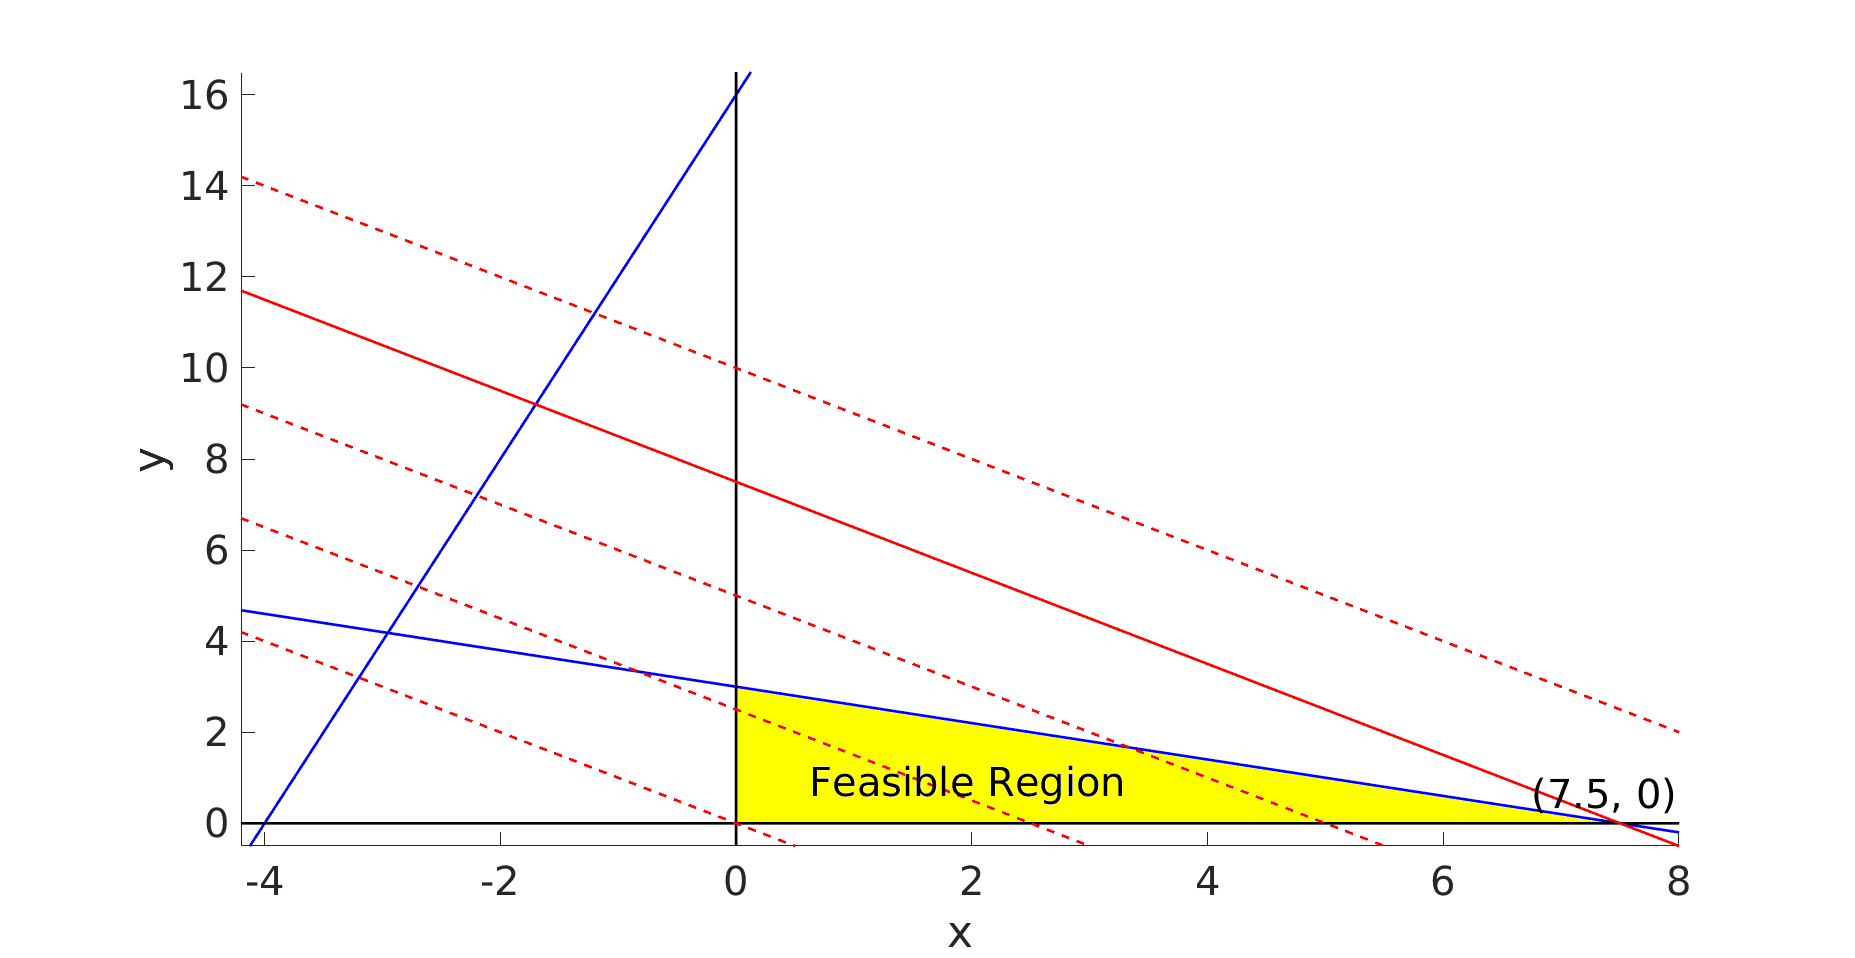
\includegraphics[width=12cm]{problem2a.png}\\
\caption{Feasible region and optimal solution of the primal problem}\label{primal}
\end{figure}

\subsection{Part (b)}
To construct the dual problem, we want to find $a$ and $b$ such that
\begin{equation*}
x+y\leqslant a(-4x+y)+b(2x+5y)=(-4a+2b)x+(a+5b)y
\end{equation*}
and we want to minimize $16a+15b$.

The dual problem is thus
\begin{align*}
s^*=\min_{a,b}~&16a+15b\\
\textup{s.t. }-4a+2b&\geqslant1\\
a+5b&\leqslant1\\
a&\geqslant0\\
b&\geqslant0
\end{align*}

A graphical solution is given in Fig.\ref{dual}. Minimizing $16a+15b$ corresponds to downwards shifting the curve $b=-16a/15+s/15$ as much as possible, while making it pass the feasible region. From the graph, the optimal solution is on a corner: $(a^*,b^*)=(0,0.5)$. The maxmized total amount of sauce is $s^*=7.5$.
\begin{figure}[!htbp]
\centering
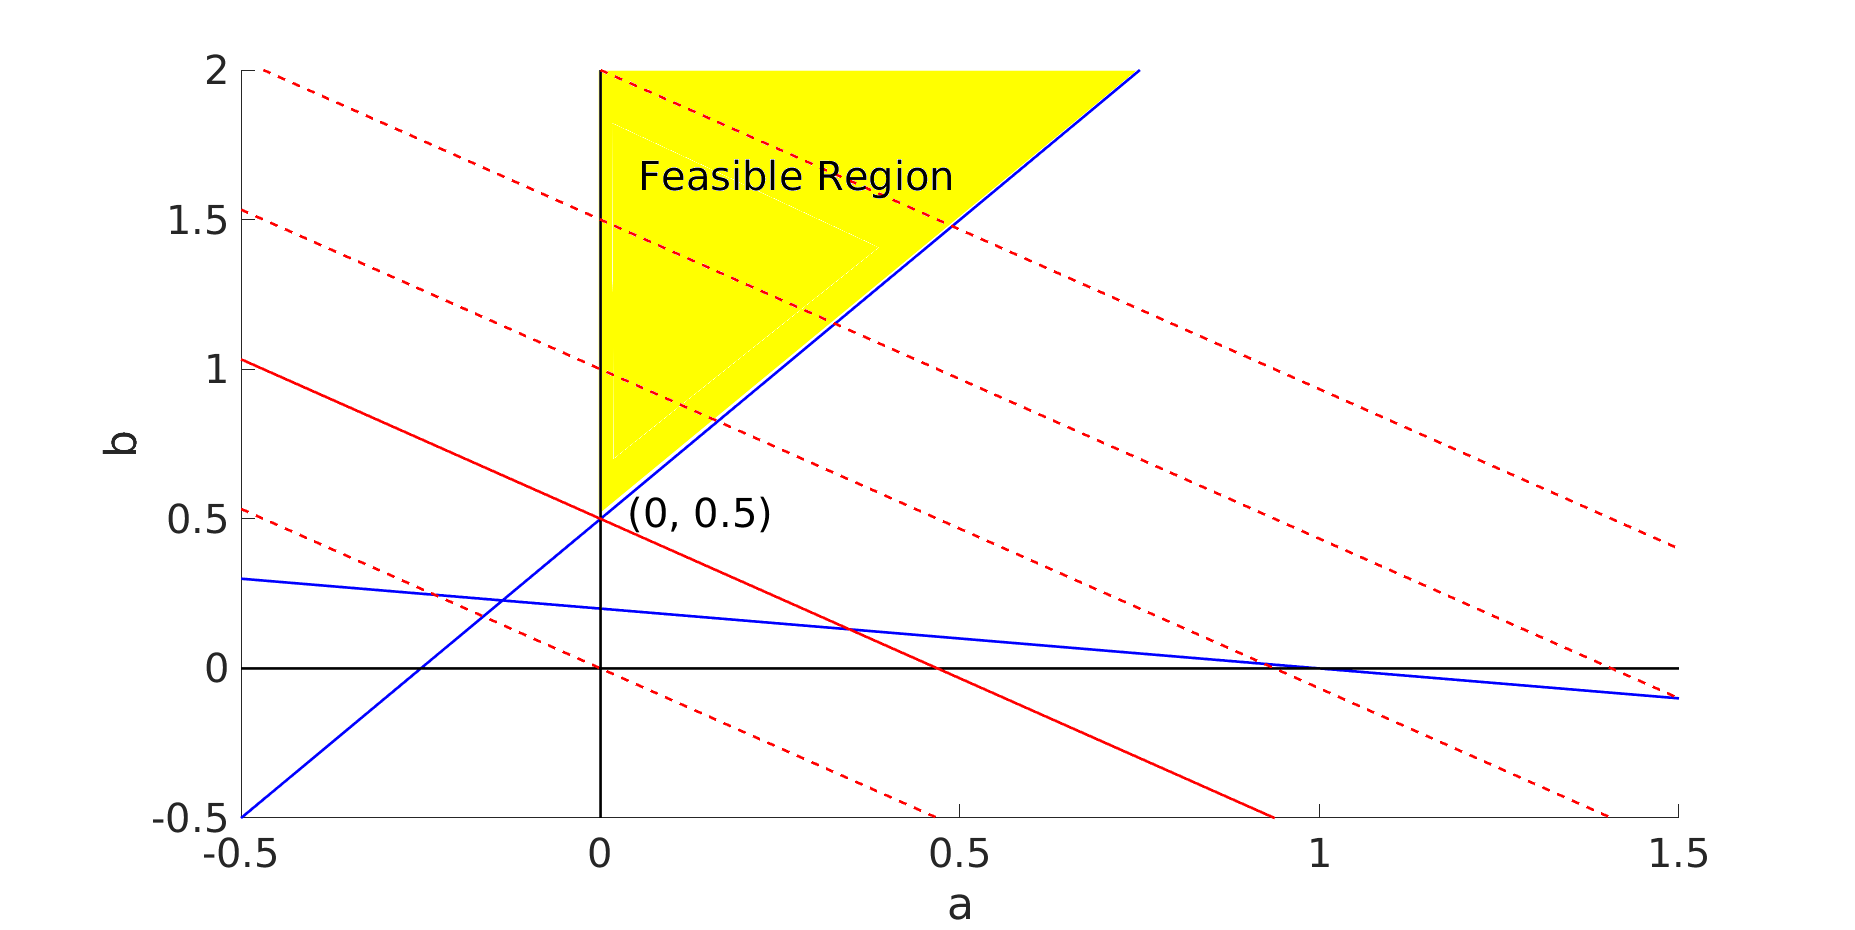
\includegraphics[width=12cm]{problem2b.png}\\
\caption{Feasible region and optimal solution of the dual problem}\label{dual}
\end{figure}

To prove optimality in part (a), notice that
\begin{align*}
x+y&\leqslant(-4a^*+2b^*)x+(a^*+5b^*)y\\
&=a^*(-4x+y)+b^*(2x+5y)\\
&\leqslant16a^*+5b^*\\
&=7.5
\end{align*}
where the first inequality uses constraints in the dual problem as well as non-negativity of $x$ and $y$, and the second inequality uses constraints in the primal problem as well as non-negativity of $a^*$ and $b^*$. Since $x+y\leqslant7.5$, the choice $(x^*,y^*)=(7.5,0)$ which makes $s^*=7.5$ must be optimal.
\end{document}
